\begin{frame}{Triangle exercise}
\begin{enumerate}
\item ABC and AMP are two right triangles, right
angled at B and M respectively. M lies on AC
and AB is extended to meet P. Prove that:
\seti
\begin{enumerate}
\item $\triangle{ABC} \sim \triangle{AMP}$
\item $\frac{CA}{PA}=\frac{BC}{MP}$
\end{enumerate}
\end{enumerate}
\textbf{Solution:}
\begin{figure}[!ht]
\resizebox{.4\linewidth}{!}
{
\begin{tikzpicture}[scale =2.5,>=stealth,point/.style = {draw, circle, fill = black, inner sep = 1pt},]
\node (C) at (4,3)[point,label=above :$C$] {};
\node (A) at (0,0)[point,label=below :$A$] {};
\node (B) at (4,0)[point,label=below :$B$] {};
\node (P) at (5,0)[point,label=below :$P$] {};
\node (M) at (3.2,2.4)[point,label=above :$\textbf{M}$] {};
\draw (A)--(B);
\draw (B)--(C);
\draw (C)--(A);
\draw (P)--(M);
\draw (B)--(P);
\tkzMarkRightAngle[fill=white!45,size=.3,mark=](C,B,A)
\tkzMarkRightAngle[fill=white!45,size=.3,mark=](A,M,P)
\end{tikzpicture}

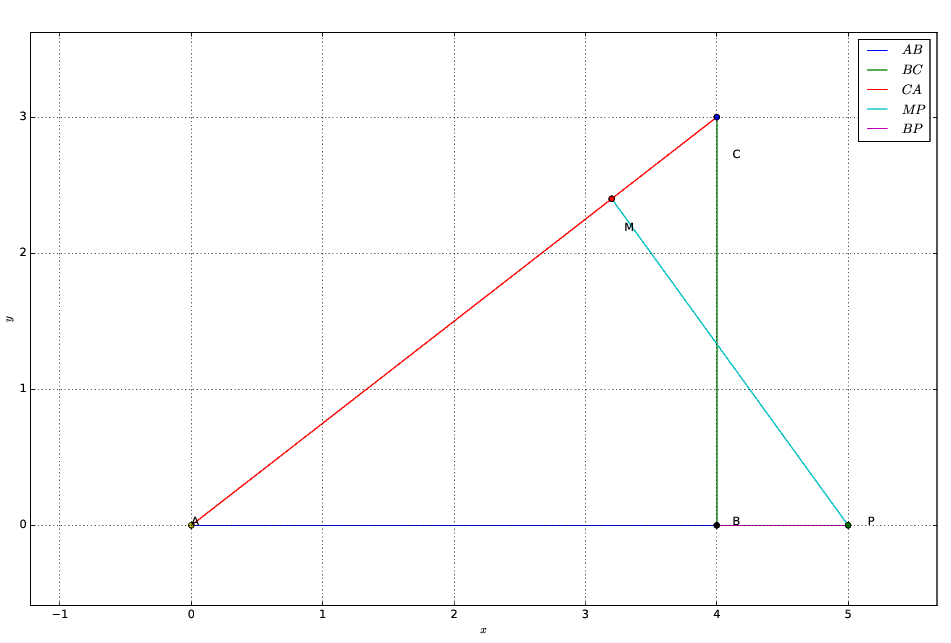
\includegraphics[scale=0.4]{./figs/triangle/tri.png}
}
\caption{right angled triangles}
\label{fig:foo}
\end{figure}
\end{frame}
\begin{frame}
From the above figure
\begin{align}
	\angle{CAB} =\angle{MAP} \\
	\angle{ABC} = \angle{AMP}
\end{align}
From 1 and 2
\begin{align}
\triangle{ABC} \sim \triangle{AMP}
\end{align}
\begin{itemize}
\item As correspondinng sides are proportional
$\frac{CA}{PA}=\frac{BC}{MP}=\frac{AB}{AM}$

\begin{center}
$\frac{CA}{PA}=\frac{BC}{MP}$
\end{center}
\end{itemize}
\end{frame}